\providecommand{\home}{../../../..}
\documentclass[\home/main.tex]{subfiles}
\usetikzlibrary{shapes,arrows,calc,positioning,fit} 


\begin{document}

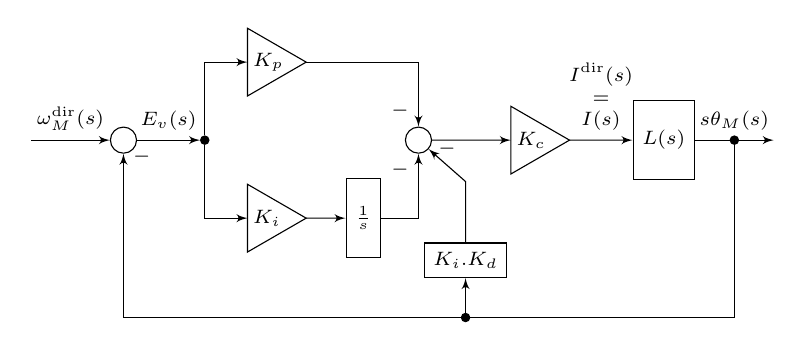
\begin{tikzpicture}[>=latex',every node/.append style=
    {font=\scriptsize},node distance=5mm]

    \tikzset{
        %   pinstyle/.style={pin edge={to-,thin,black}}, % you have another one below
           block/.style = {draw, rectangle,
               minimum height=1cm,
               align = center
            %   minimum width=2cm
           },
           input/.style = {coordinate,node distance=1cm},
           output/.style = {coordinate,node distance=1cm},
           arrow/.style={draw, -latex,node distance=2cm},
           pinstyle/.style = {pin edge={latex-, black,node distance=2cm}},
           sum/.style = {draw, circle, node distance=1cm},
           gain/.style = {
             regular polygon, regular polygon sides=3,
             draw, fill=white, text width=1em,
             inner sep=0mm, outer sep=0mm,
             shape border rotate=-90
           },
           dot/.style={circle,fill,draw,inner sep=0pt,minimum size=3pt}
         }

    %DEFINIZIONE BLOCCHI
    \node [input, name=input] {};
    \node [sum, right=of input] (speed_sum) {};
    \node [dot, right=8mm of speed_sum] (snodo1) {};
    \node [gain, above right=7mm and 5mm of snodo1] (Kp) {$K_{p}$};
    \node [gain, below right=7mm and 5mm of snodo1] (Ki) {$K_{i}$};

    \node [block,right=of Ki] (integrator) {$\frac{1}{s}$};
    \node [sum, xshift=7mm] at (snodo1-|integrator) (control_sum) {};
    \node [gain, right=1cm of control_sum] (Kc) {$K_{c}$};
    \node [block, right=8mm of Kc] (system) {$L(s)$};
    \node [output, right=of system] (output) {};


        %DEFINIZIONE COLLEGAMENTI IN CATENA DIRETTA
    \begin{scope}[auto]
    \draw [->] (input) -- node {$\omega_{M}^{\mathrm{dir}}(s)$} (speed_sum);
    \draw [->] (speed_sum) -- node {$E_{v}(s)$}(snodo1);
    \draw [->] (snodo1) |- (Kp);
    \draw [->] (snodo1) |- (Ki);
    \draw [->] (Ki) -- (integrator);
    \draw [->] (Kp) -| (control_sum) node[very near end,swap] {$-$};
    \draw [->] (integrator) -| (control_sum) node[very near end] {$-$};
    \draw [->] (control_sum) -- (Kc);
    \draw [->] (Kc) -- node [align=center] {$I^{\mathrm{dir}}(s)$\\$=$\\$I(s)$}(system);
    \draw [->] (system) -- node [name=motor_speed] {$s\theta_{M}(s)$}
        (output);
    \end{scope}

        %DEFINIZIONE COLLEGAMENTI FEEDBACK
    \draw [->] (motor_speed) -- ++ (0,-2.5) -| node [pos=0.99,right] {$-$} node[dot,pos=0.22] (snodo2) {}
    (speed_sum);
    \node [dot] at (motor_speed.south) {};

    \draw [->] (snodo2) -- ++(0,0.5) node[above,draw] (KiKd) {$K_i.K_d$};
    \draw [->] (KiKd) -- ++(0,1) -- node[above,pos=0.5] {$-$}(control_sum);

\end{tikzpicture}

\end{document}
